\documentclass[11pt,a4paper]{report}

\usepackage[utf8]{inputenc}
\usepackage{lmodern}

\usepackage{fullpage}

\usepackage{amsmath, amsfonts, amssymb, amsxtra}

\usepackage{tikz}
\usepackage{graphicx}
\graphicspath{{./fig/}}
\usepackage[svgpath=fig/]{svg}

\usepackage{listings}

\usepackage{natbib}

\newtheorem{theorem}{Theorem} 
\newtheorem{definition}[theorem]{Definition} 
\newtheorem {folgesatz}[theorem]{Folgesatz}

\begin{document}
 \title{Automatic Speech Recognition for PR2 Robotic Control under ROS} 
\author{Weipeng He, Natalia Orlova \\ \\
\small Report in Masterproject Intelligent Robotics, WS 2013/2014\\
Department of Informatik\\ Hamburg University\\[4mm]}
\maketitle

\begin{abstract}
  In this report we would like to present the theories and implementations of our speech recognition system on PR2. 
\end{abstract}

\tableofcontents

\chapter{Introduction}
\label{sec:intro}

\section{Motivation}
Speech is a unique mechanism, that to a great extent makes human
communication possible. However, there are many spoken situations, in which
the meaning of  either similarly pronounced or  not clearly
articulated words is not obvious due to different reasons, like noise, accent,
speaker's age, background, etc. One straightforward example is  a phrase \textit
{It is not easy to recognise speech} . It could be simply misheard as \textit
{It is not easy to wreck a nice beach} or \textit {It not not easy to wreck an
ice beach}.

 No wonder, that research on speech complexity and
ambiguity requires sophisticated scientific analysis and studies. Only full 
understanding of this communicative means as a phenomenon enables the 
knowledge transfer to the areas of technology, where speech builds a natural
 interface between humans and machines.  Automatic speech recognition in the 
 environment of a human-machine interaction  is a challenging implementation and
 research task, that brings to live natural and user-friendly means of communication with electronic devices and robots. 

\section{Problems and Questions of the Project}
Intelligent Robotics at Hamburg University is one of the projects, aimed at
research of artificial intelligence and development of human-machine 
interfaces and applications for service robots. This report is mainly dialed
with the speech recognition issues of the project. In the \textit {speech
recognition} part of the project we are mainly focused on a robot speech control, the study of sound source separation and the possible 
integration of a 
noise filter with a normal recogniser. The
practical part is aimed at the development of a command-driven application  for
a service robot, involving analysis of its performance. 

\section{Report Layout}
The report consists of the following parts. The chapter ~\ref {sec:intro}
contains introduction, presenting the main tasks of the \textit {speech
recognition} project part. The chapter ~\ref {sec:overview} gives a brief
description of the project ant determines the place of the \textit {speech
recognition} part in it.  The main focus of the chapter ~\ref {sec:architecture} is the architecture of a typical
speech recogniser, description and relations of its main components. 
Chapter ~\ref {sec:PR2} contains details of the of the speech control
implementation for PR2 service robot under ROS. Chapter \ref{sec:noise}
shows the possibilities and advantages of a noise reduction in speech
recognition. It deals with two problems: sound source separation and spectral subtraction techniques.
The closing chapters \ref{sec:results} and \ref
{sec:conclusion} presents results of \textit{speech recognition} project part
and summarize the key ideas of the report.

\chapter {Project Overview}
\label {sec:overview}

The aim of the project is an implementation of an integrated
application for a PR2 service robot under ROS.  The project
consists of the following separate, but closely connected parts: \textit {speech
recognition}, \textit {gesture recognition} and \textit {object recognition}.
The final application has the following scenario.  The commands in the forms of
words or gestures are processed by a command handler and sent to the robot for execution.  The first aim is 
to map a gesture or a voice command to the string of words, that can
be used for further execution. This is done either by the \textit  {speech} or
\textit {gesture recognition} part, depending on the way the command is given.

 
The number of commands is limited and identical for the \textit
{speech} and \textit {gesture recognition} parts. Decoded commands are published
to the topic, to which the command-handler is subscribed.  The commands 
contain references to the objects, that the robot should be able to detect via
a built-in camera. Correct detection of the objects, mentioned in a command,
guarantees correct calibration and execution of the command. The last is the task of the \textit {object recognition} part. 

 \textit {Speech recognition} part of the project, in its turn,
can be divided in two logical parts. The first one is dealing with general questions of
a speech recogniser design and architecture and implementation of a speech
recogniser for robot control. The second logical part is focused on the
problems of a noise reduction and the use of sound separation techniques for
speech recognition. 


\chapter{Speech Processing Basics}

\section{Implementation of Audio I/O System}
Although there are plenty of literatures about the theories of audio processing, there rarely are detailed documents on how the systems are implemented. To close the gap between theories and implementation, in this section, we would like to address the basic concepts of audio programming as well as details of the implementation of basic audio input and output in our system.

Theories of audio processing are always seemed to be neat and appealing. However, when it comes to writing a program to realize an algorithm, much more ``dirty'' works will be involved. These extra works are largely due to handling of hardware status and numerical computing, which are sometimes neglected in theories.

In this section, we will first introduce the basic concepts of digital audio signal processing. Afterward, we will show how to implement a minimal audio recording program using the Advanced Linux Sound Architecture (ALSA).

\subsection{Sampling and PCM}
To process an audio signal, first of all, we need to know how the signal is represented. Ideally, the audio signal is just amplitudes over time (time-domain signal), namely $ x(t) \in \mathbb{R},~ t \in \mathbb{R} $. However, practically, we need to represent the signal discretely. Thus, discretization on both time and amplitude (\textit{sampling} and \textit{quantization}, respectively) should be applied. As the result, the signal is represented using a sequence of quantized values $x_n$.

For sampling, we take the values of the continuous signal using a \textit{sampler} at $T_s$ time intervals: \[ x_s[n] = x(n T_c) \in \mathbb{R},~ n \in \mathbb{Z} \] Here, $T_s$ is called the \textit{sampling period}, and $ f_s = \frac{1}{T_c} $ is called the \textit{sampling frequency}.

After sampling, the \textit{A/D converter} converts the real values to a limited set of values, which can be represented by binary data. In digital audio, \textit{Pulse-code modulation} (PCM) is the most common method for this quantization process. 

PCM has several quantization methods, which includes Linear PCM, A-law algorithm or $\mu$-law algorithm. Although different algorithms exist, PCM sometimes refer to Linear PCM by default as it is the most popular. Linear PCM quantize each sample using linearly uniform levels. In other words, all adjacent levels have the same difference in sound amplitude. The number of levels depends on the bit depth of each code. Figure \ref{fig:pcm} shows the sampling and quantization process using a 4-bit Linear PCM.

\begin{figure}[htbp]
  \centering
  \includesvg[pretex=\footnotesize,width=.6\textwidth]{pcm}
  \caption{Sampling and quantization process of a sine wave usineg a 4-bit Linear PCM. First, the sine wave (red curve) is sampled at discrete time (vertical lines). After that the value is rounded to the nearest possible value (blue dots). The number of possible values (horizontal lines) are $2^4=16$, and consecutive values have the same difference.}
  \label{fig:pcm}
\end{figure}

Within each quantization method, different encoding method, e.g. \textit{format}, can be chosen. These formats are named according to the bit depth, endianness, float/integer and signed/unsigned that they use. For example, a format can be 32 bits signed integer with little endian. Some applications and libraries, such as aplay, ALSA, gstreamer, use a short name for each format. As for the example format, the name is ``\texttt{S32\_LE}''. The structure of the format name is shown in Figure \ref{fig:pcmname}. Other common formats includes \texttt{S8}, \texttt{U8}, \texttt{S16\_LE}, \texttt{F32\_LE}, \texttt{F64\_LE}, etc.

\begin{figure}[htpb]
\begin{center}
  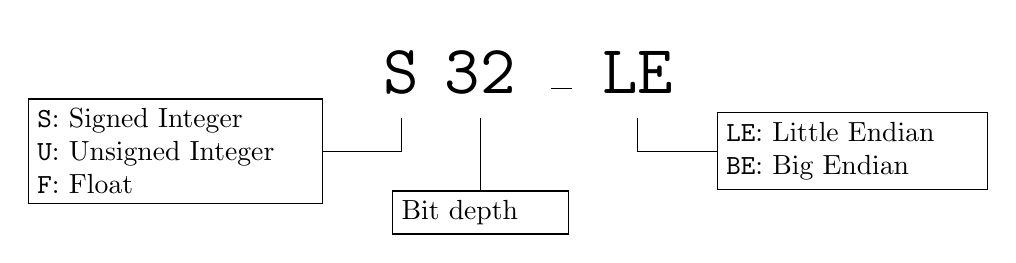
\begin{tikzpicture}
    {\Huge\texttt{
      \node(s) at (0,0) {S};
      \node(b) at (1,0) {32};
      \node at (2,-0.2) {\_};
      \node(e) at (3,0) {LE};
    }}
    \draw (-1,-1) node[left,text width=3.5cm,draw,rectangle]
       {\texttt{S}: Signed Integer\\\texttt{U}: Unsigned Integer\\\texttt{F}: Float} -| (s.south);
    \draw (1,-1.5) node[below,text width=2cm,draw,rectangle]
       {Bit depth} -- (b.south);
    \draw (4,-1) node[right,text width=3.2cm,draw,rectangle]
       {\texttt{LE}: Little Endian\\\texttt{BE}: Big Endian} -| (e.south);
  \end{tikzpicture}
\end{center}
\caption[Name structure of PCM format.]{Name structure of PCM format. The first letter represents the data type. Then follows a number, which is the bit depth of each sample. If the bit depth is larger than 8 (1 byte), then there is a tag, which states the endianness, at the end.}
  \label{fig:pcmname}
\end{figure}

Now, we can represent a single channeled audio recording using a sequence of PCM binary data. Furthermore, for multi-channeled audio recording, it it just simple interleave the data of each channel. A set of samples at one time from all channels is called a \textit{frame}. For example, suppose we have a 2-channeled data using \texttt{S16\_LE} format. Then the first 2 bytes are the first sample of channel 1, and the second 2 bytes are the first sample of channel 2. Thus, bytes number 1 to 4, are the first frame. And, the second samples of both channels are at the number 5 to 8 bytes, which consist the second frame. And so on.

To summarize, an audio recording can be represented by binary data using PCM. To sufficiently understand how the audio are encoded, we need to know the following parameters: sampling rate, number of channels and PCM format.

\subsection{Advanced Linux Sound Architecture}
Advanced Linux Sound Architecture (ALSA) is the software framework that provides API for sound device drivers as part of the linux kernel. The API includes configuration of the hardware and write/read audio data.

Besides the aforementioned parameters for audio representation (sampling rate, number of channels and PCM format), some other parameters regarding the hardware buffer are also need to be configured. These parameters are period size and buffer size. As it could be very costly for CPU to fetch the data one sample at a time, normally there is a hardware interrupt every interval. The number of frames that is in this interval is called the \textit{period size}. These data are stored in a ring buffer, and its size if called \textit{buffer size}. Usually the buffer size is twice as the period size. However, it can sometimes be up to 8 times of that.

% \subsection{Implementation using ALSA}

\section{Short Time Fourier Transform}
In previous section, we introduced the basics about speech signal in time domain. However, it can be difficult to analyze the time-domain signal. By using Fourier transform, we can change the signal to frequency domain and benefit from its several properties. Still, the problem for Fourier transform is that the speech signal is quasi-stationary (slowly varying over time) rather than stationary. Which means frequency-domain signal cannot specify the local information at a specific time. Therefore, the \textit{Short Time Fourier Transform} (STFT) is applied, in order to modeling the signal in both time and frequency domains.

\subsection{Window Function}
In STFT, the idea of ``short time'' is realized by applying a window function to the original signal at a specific time. Window function is zero-centered and non-zero in only a short interval. Typical window functions include: Hann window, Hamming window\cite{heinzel_spectrum_2002}. The Hann window (Figure \ref{fig:hann}) is defined as:
\[ w(n) = 0.5 (1 - \cos(\frac{2\pi n}{N-1})) \]
and Hamming window (Figure \ref{fig:hamming}) is defined as:
\[ w(n) = \alpha - \beta \cos(\frac{2\pi n}{N-1}) \]
where $\alpha = 0.54, \beta = 1 - \alpha = 0.46$ and $N$ is the window size.

\begin{figure}[htbp]
  \centering
  \includesvg[pretex=\footnotesize,width=.8\textwidth]{hann}
  \caption[Hann Window]{Hann Window.}
  \label{fig:hann}
\end{figure}

\begin{figure}[htbp]
  \centering
  \includesvg[pretex=\footnotesize,width=.8\textwidth]{hamming}
  \caption[Hamming Window]{Hamming Window.}
  \label{fig:hamming}
\end{figure}

\subsection{Continuous STFT and its Inverse}
Continuous STFT is simply traditional Fourier transform applied to windowed signal. Mathematically, continuous STFT is expressed as:
\[ X(\tau, \omega) = \mathcal{F}(x(t)w(t-\tau)) =  \int_{-\infty}^{\infty} x(t)w(t-\tau)e^{-j\omega t}\mathrm{d}t \]
where $\mathcal{F}$ is the Fourier transform, $x(t)$ is the time-domain signal to be transfered and $w(t)$ is the window function. For a fixed time $\tau$, $x(t)w(t-\tau)$ is just the original signal at local time around $\tau$ and masked by the window function. Thus, $X(\tau, \omega)$ represents the frequency attributes at that local time. We can also notice that the transform $X(\tau, \omega)$ depends on both time $\tau$ and frequency $\omega$. Therefore, we say that this kind of representation the time-frequency representation.

Like Fourier transform, the continuous STFT is invertible. Now we show how the inverse transform is derived. First, we assume the window function is scaled to have $\int_{-\infty}^{\infty} w(t) \mathrm{d}t = 1$. Thus:
\[
  x(t) = x(t) \int_{-\infty}^{\infty} w(t-\tau) \mathrm{d}\tau = \int_{-\infty}^{\infty} x(t)w(t-\tau) \mathrm{d}\tau
\]
The integrand $x(t)w(t-\tau)$ is actually the original signal of $X(\tau, \omega)$ before Fourier transform with $\tau$ fixed. Therefore:
\[ x(t)w(t-\tau) = \mathcal{F}^{-1}(X(\tau, \omega)) = \frac{1}{2\pi} \int_{-\infty}^{\infty} X(\tau, \omega) e^{j\omega t} \mathrm{d}\omega \]
Combining the two equations above, we have the inverse of the transform:
\[ x(t) = \frac{1}{2\pi} \int_{-\infty}^{\infty} \int_{-\infty}^{\infty} X(\tau, \omega) e^{j\omega t} \mathrm{d}\omega \mathrm{d}\tau \]

\subsection{Discrete STFT}
Because we don't have continuous speech signal, we shall extend the STFT to discrete situation\footnote{Most time, without specification, STFT means discrete STFT by default.}. Like the discrete Fourier transform (DFT), discrete STFT is defined as:
\[ X(n, k) = \sum_{m = -\infty}^{\infty} x[m]w[m-n]e^{-j \frac{2\pi k}{N} m} \]
where $x$ is the signal, $w$ is the window function, $n$ is the index of time, $k$ is the index of frequency bin, and $N$ is the number of frequency bins. Practically, most applications of STFT use Fast Fourier Transform to calculate. Thus, the $N$ is also equal to the window size and is an exponential of 2.

The magnitude squared of the STFT yields the spectrogram of the function:
\[ \text{Spectrogram}(n, k) = \left|X(n,k)\right|^2 \]
From the spectrogram we can clearly visualize the different frequency components of a sound and its variation over time. In fact, most application for extracting audio feature use only the magnitude information.

Note that because the time-domain signal is real, at any time, the result of the DFT has the following properties:
\begin{itemize}
  \item $X(n,0)$ and $X[n, \frac{N}{2}]$ are real;
  \item $X(n,k) = X^*(n,N-k), k \neq 0, \frac{N}{2}$, here $^*$ is the complex conjugate.
\end{itemize}
Therefore, only the first half (index from $0$ to $\frac{N}{2}$) of the DFT contains information, while the other half are redundant. In fact, only the first half is plotted in the spectrogram. From Fourier analysis theories, we know that the $k$th frequency bin represents the component at frequency $\frac{kf_s}{N}$, with $f_s$ is the sampling rate. The component with the highest frequency is the bin with index $\frac{N}{2}$ and its frequency is $\frac{N}{2} \times \frac{f_s}{N} = \frac{f_s}{2}$. This is consistent with the Nyquist frequency.

One shortcoming for STFT is that the frequency resolution and time resolution is mutually limited. This limit is referred as \textit{Gabor limit}. The difference of two consecutive frequency bin is $\frac{f_s}{N}$. And, one STFT is a DFT of a neighborhood of $N$ samples, e.g. $N * \frac{1}{f_s}$ time interval. That means the time resolution is $\frac{N}{f_s}$. Therefore, the product of the two resolutions, $\frac{f_s}{N} \times \frac{N}{f_s} = 1$, is constant. Selecting the windows size involves trade-off between the frequency resolution and time resolution. With large window size, we can have good frequency resolution, while it can be difficult to catch the change in a short time. Vice versa, with a small windows size, we can have high time resolution. However, the frequency resolution would be low.

\subsection{Inverse Discrete STFT}
Because DFT is invertible, calculating the inverse of STFT can be quite direct. For any $n$, we can find $m$, such that $w[n-m] \neq 0$. We have:
\[ x[n]w[n-m] = \mathcal{F}^{-1}(X(m,k))[n] \]
where $\mathcal{F}^{-1}$ is the inverse DFT. Thus,
\begin{equation}
  x[n] =  \frac{\mathcal{F}^{-1}(X(m,k))[n]}{w[n-m]} = \frac{\frac{1}{N}\sum_{k=0}^{N-1} X(m,k)e^{j \frac{2\pi k}{N} n}}{w[n-m]}
  \label{eq:naiveinv}
\end{equation}

We can clearly see that there could be multiple $m$, which yields the same result. In other words, the STFT is redundant. Therefore, except for calculating every $n$, we jump a interval between calculation of DFT. Which means, we use a shifting window, that shift more than 1 sample a time. With the \textit{shift size} $L$, we calculate the STFT at time $0$, $L$, $2L$, \dots. Thus, we can have windows that covers $[0, N-1]$, $[L, L+N-1]$, $[2L, 2L+N-1]$, \dots. In order to cover all samples, we need $L<N$, which means we have overlapping windows. Normally, we choose $L = \frac{N}{2}$ or $L = \frac{N}{4}$. Figure \ref{fig:window} shows two situations. In the first figure, where shift size is half of the window size, we can see that every sample is covered by at least one window. However, in the second figure, where the shift size if large than window size, there is intervals between consecutive windows. The samples in such intervals cannot be inversed, because whatever their values are, after windowing, their value will be zero. 

\begin{figure}[thbp]
  \centering
  \includesvg[pretex=\footnotesize,width=.6\textwidth]{window}
  \caption{Shifting Window (size $N$) with different Shift Size ($L$).}
  \label{fig:window}
\end{figure}

Although Equation \ref{eq:naiveinv} can still be used for calculating the inverse, it is not a good practice. It is because the $w[n-m]$ in the denominator can be very small, which amplifies small perturbation in the STFT. One of the algorithms to solve this issue is called the \textit{Overlap-add} (OLA) method.

The idea of OLA is simply calculating the inverse of all window frames and take the weighted average of them. The inverse is calculated as:
\begin{equation}
  x[n] = \frac{\sum_{p=-\infty}^{\infty} \mathcal{F}^{-1}(X(pL,k))[n]}{\sum_{p=-\infty}^{\infty} w[n-pL]}
  = \frac{\sum_{p=-\infty}^{\infty} \sum_{k=0}^{N-1} X(pL,k)e^{j \frac{2\pi k}{N} n}}{N\sum_{p=-\infty}^{\infty} w[n-pL]}
\end{equation}

Under some constraint, $\sum_{p=-\infty}^{\infty} w[n-pL] = W_0$ is constant. Then the inverse STFT is:
\begin{equation}
  x[n] = \frac{1}{NW_0} \sum_{p=-\infty}^{\infty} \sum_{k=0}^{N-1} X(pL,k)e^{j \frac{2\pi k}{N} n} 
  \label{eq:olainv}
\end{equation}

Now, we have shown that OLA can be used for calculating the inverse of STFT.

\chapter {Architecture of Speech Recognition}
\label {sec:architecture}

Contemporary speech recognisers are complex systems, built of
numerous components. However, prior to the architecture analysis, it is necessary to give
a definition of an automatic speech recognition. \begin {definition}[Automatic speech recognition] building of a
system for automatic mapping of an acoustic signal to a string of words. \citep
{jurafsky-martin-2009}.
\end{definition}
\begin  {figure}[h]
\begin {center}
     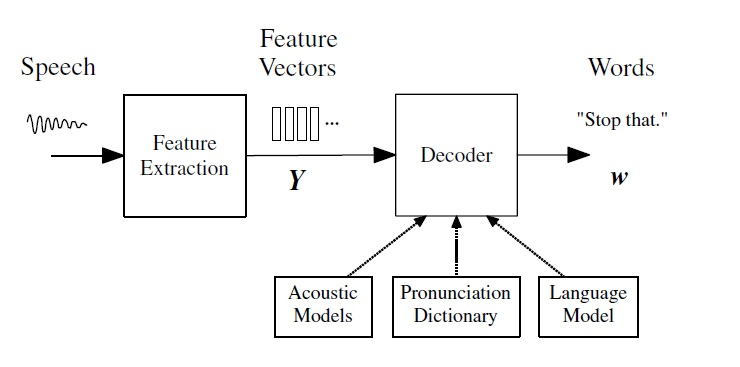
\includegraphics[height=6.0 cm]{arc2}
     \caption {Speech recogniser architecture \citep {Gales2008application}.}
     \label {fig:arc}
     \end {center}
     \end {figure}

As it can be seen from the figure \ref{fig:arc} a typical
speech recogniser consists of the following components: acoustic analysis, acoustic model,
language model and decoder, getting as an input acoustic vectors and the results
of acoustic and language modeling and producing a decoded string sequence as
an output.  In the next sections the components of a speech recogniser are
analysed in more details. 

\section {Acoustic analysis}
In a physical sense human speech is a sound wave, characterized by a
particular amplitude, frequency, period and length. 
\begin  {figure} [h]
\begin {center}
     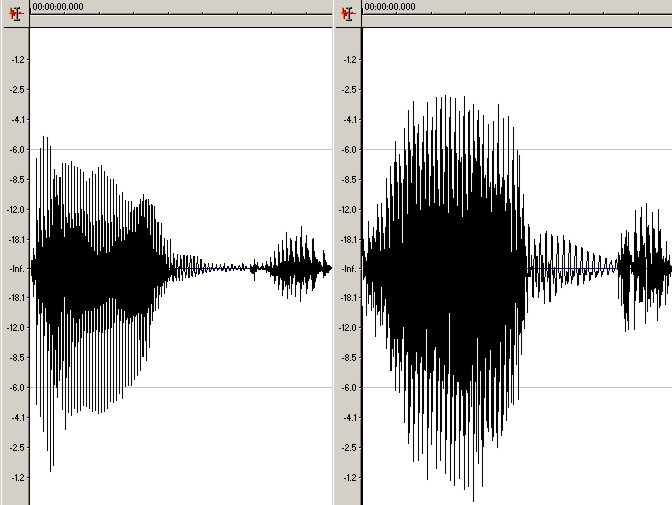
\includegraphics[height=5.0 cm]{egg}
     \caption {The wave representation of the word egg, pronounced by European
     and non-European native speaker \citep{SpeechRecognition}.}
     \label {fig:egg}
     \end {center}
     \end {figure}

 In the figures ~\ref{fig:egg} and ~\ref{fig:hamburger} the
sound waves of the words \textit {eggs} and \textit{hamburger}, pronounced by
European and non-European test speakers are shown. As at can be seen from this examples the waveforms of the word \textit {hamburger}
produced more similarities then the waveforms of a short word \textit {egg}. 
Figure ~\ref{fig:egg-bread} illustrates that pronunciation of different words
may also lead to similar waveform signals. Obviously, similar examples
(compare figures ~\ref{fig:egg} and ~\ref{fig:egg-bread}) produces difficulties
for artificial recognition systems during decoding. 
 \begin  {figure} [h]
\begin {center}
     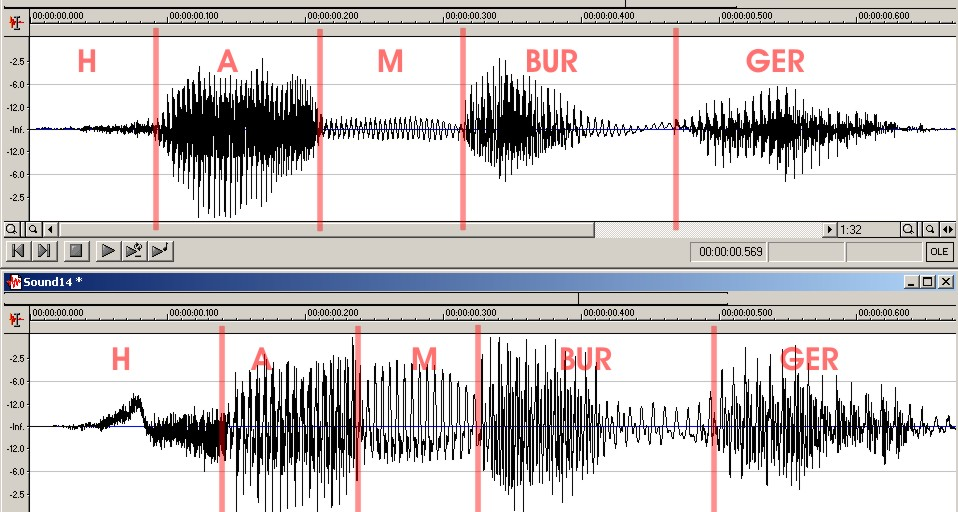
\includegraphics[height=5.0 cm]{hamburger}
     \caption {The wave representation of the word hamburger, pronounced by the
     same European and non-European native speaker \citep
     {SpeechRecognition}.}
     \label {fig:hamburger}
     \end {center}
     \end {figure}
\begin {figure} [h]
     \begin {center}
     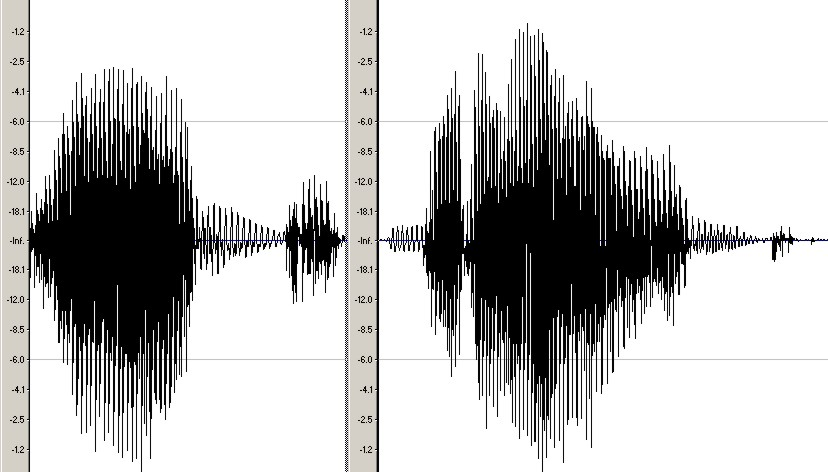
\includegraphics[height=5.0 cm]{egg-bread}
     \caption {The wave representation of the words egg and bread, pronounced
     by the same person\citep
     {SpeechRecognition}}.
     \label {fig:egg-bread}
     \end {center}
     \end {figure}

 
Decoding is preceded by features extraction and digitalizing of a
signal signal in such a way, that mathematical operations and calculations are
made possible. Preprocessing of speech as an analogous signal demands the
following steps. First, the waves are sampled, which allows getting a discrete signal from the continuous one. Second, the 
samples are quantized, mapping the analog values to digitalised ones. Third,
a digital signal is converted to its spectral representation, applying a
short-time Fourier transform. The resulting sound spectrum  contains the amount of vibration at each individual frequency. Figure ~\ref {fig:spectrum} shows a typical spectral representation
of word. 

 Finally, with the help the sound spectral
representation acoustic vectors of features \textbf {Y}(compare figure ~\ref
{fig:arc}) are created. One of the most commonly used for this purpose method is a mel-frequency cepstrum (MFC). This
method calculates coefficients representing the amplitudes of the
resulting spectrum, so-called mel-frequency cepstrum coefficients (MFCC).
Resulting acoustic vectors of features are used as a representation of a
sound waveform, forwarded to the decoder for recognition. 
 \begin {figure} [h]
     \begin {center}
     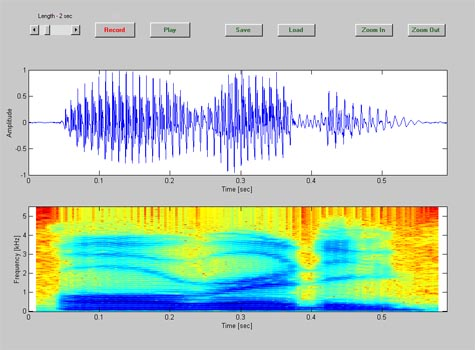
\includegraphics[height=6.0 cm]{already}
     \caption {Waveform and spectrogram of the word already \citep {hansen}}.
     \label {fig:spectrum}
     \end {center}
     \end {figure}

\section {Acoustic model}
Acoustic model finds out the probability for a a given acoustic vector \textbf
{Y} to be mapped to a known sequence of words \textbf {P(Y(W))}. For a small
vocabulary it can be found by sampling several variants of the words and
computing statistical similarity of the inputs with the existing samples.
However, when the vocabulary is very large we have to move down to the level of
word subunits. 

 All the words in the language consist of phonemes, small
pronunciation units, which combinations and positions influence the change of meaning. The number
of the phonemes differs in different languages. For example, in English the
number of phonemes varies, depending on a dialect.  Some English dialects
have only 40 phones, other about 50. 

 
Acoustic model contains statistical representation of each
phoneme in the form a Hidden Markov Models (HMM). HMM is a state automate with probabilistic
parameters.

A typical HMM is depicted in the figure
~\ref{fig:hmm}.  This HMM for phoneme recognition has 3 states  S0, S1, S2.
Letters 'A' shows the transition probabilities within the states, 'B' - output
probabilities, 'Y' -observations. Number of HMM states can vary depending on
implementation. Implementations with 3-5 states are most common. Word
representations in acoustic model forms a network of HMMs.  
\begin {figure} [h]
  \begin {center}
    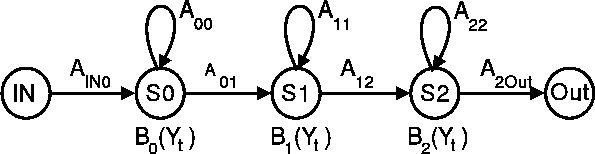
\includegraphics[]{HMM}
    \caption {Hidden Markov Model for phoneme recognition \citep{jurafsky-martin-2009}}.
    \label {fig:hmm}
  \end {center}
\end {figure}
  Acoustic models are created from an hours-long audio recordings and
their corresponding transcriptions. In order to get a statistical
representation of phonemes, i. e, build HMM for each phoneme, the speech corpus
data is subjected to the training process.  

 Speech corpus
data and resulting models differs in speech parameters: microphone speech, broadcast speech,
conversational speech, telephone speech. Too general models are not applicable
for more specific  language conditions, whereas too specific models are limited
in its usage. The  right choice of the acoustic model increases performance
of a recogniser. To match specific conditions of an application an
acoustic model model should be trained respectively, providing enough training
data is available. 

\section {Language model}
Language model describes the probability of a word in a speech sequence
(\textbf{P (W)}) and attempts to predict the next word in a sentence, depending
on the prior context. 

 Language models are based on n-gram sequences of words, where
the number of words of the prior context is equal n-1. The most widely used sequence is
tri-gram. An extract from a language model is shown in the listing ~\ref{L1}.
Symbols \texttt{<s>} and \texttt{</s>} means the start and the end of an utterance respectively,
and the figures - the probability of a tri-gram occurrence. 

\lstinputlisting{nav_commands.lm}
\begin{lstlisting}[caption=An extract from a language model, label=L1]
\end{lstlisting}

Language models are built on a basis of an application corpus. Corpus contains
a list of sentences that are used to train the language model.  The best
results are achieved, when the model is tuned the application speech situation.
Language models for telephone conversations are not effective for robot
instructions. 

Pronunciation dictionary also belongs to the language model. It is made of all
occurred  in the application words and their transcriptions.
Pronunciation dictionary is used by the decoder during word identification as a
reference. A typical transcription file is shown in the listing  ~\ref{L2}.

\lstinputlisting{nav_commands.dic}
\begin{lstlisting}[caption=Pronunciation Dictionary, label=L2]
\end{lstlisting}

The dictionary can be maid manually according to  transcription conversions, 
or alternatively using generators.  Some words in the
dictionary can have several possible transcriptions. On the other hand,
differently written words may sound identically (compare homophones \textit
{TO} and \textit {TWO}) from the listing ~\ref{L2}. Difference between the
homophones is only evident within context. Distinction of, for example, such
homophones as \textit {ice-cream} vs. \textit {I scream}, \textit {real eyes}
vs. \textit{realize} vs. \textit {real lies}, \textit {addressed mail} vs.
\textit {a dressed male}, etc.  is a really challenging task for an ASR,
especially when the context is not clear.  
\section {Decoder}
Speech recognition decoder receives data from acoustic inputs, acoustic and
language models and returns the most probable word sequence. The task that
the decoder is solving can be formulated in plain text as follows \textit {What
is the most likely sentence out of all sentences W in the language $\mathcal
{L}$ given some acoustic input Y?} In the terms of mathematics we are dealing
with an optimisation problem, formulated with a Bayes decision rule \citep
{jurafsky-martin-2009}:
\begin {center}
$w_{opt}=argmax \quad P(W|Y)=\frac{P(Y|W)P(W)}{P(Y)}=argmax\quad P(Y|W)P(W)$
\end {center}
Decoder solves the above optimisation problem, involving complicated search
algorithms. One of the most commonly used for speech recognition algorithm is 
Viterbi algorithm.  Viterbi is a dynamic programming search algorithm.  
It traverses the network of HMM states and finds the path with the best score.
\begin 
{figure}[h]
\begin {center}
     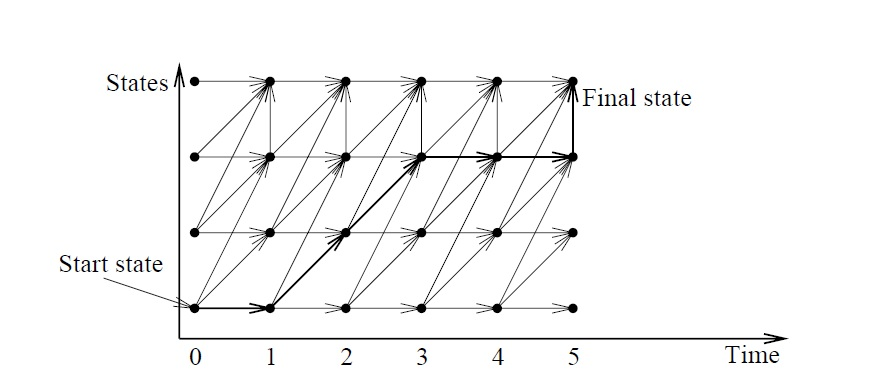
\includegraphics[height=7.0 cm]{viterbi}
     \caption {Viterbi Search as Dynamic Programming
     \citep{Ravishankar96efficientalgorithms}}
     \label {fig:viterbi}
     \end {center}
     \end {figure}
  
  Abstract representation of the Viterbi algorithm is shown in
  the in the figure ~\ref {fig:viterbi}. One axis represent states in the HMM network,
  another time.  Arrows means transitions  through the network. Each point in this 2-D space represents the best path
probability for the corresponding state at that time. Every state has a best predecessor and starting from the final state and
using backtracking it is possible to find the best path sequence for the whole search. 

 Complexity of
Viterbi algorithm is equal N$^2$ T, where N is the total number of states and
T is the total duration.  \citep{Ravishankar96efficientalgorithms}.  

 Apart from Viterbi algorithm there exist also other decoding
strategies, like stack decoding \citep{Ravishankar96efficientalgorithms} or a combination of 
several strategies.  However, analysis of these algorithms lays beyond the scope
of the current report. 


\chapter {Speech control for PR2 robot  under Robot Operation System (ROS)}
\label {sec:PR2}

The task of the \textit{speech recognition} part of the Project was development
and performance analysis of a command driven application for a PR2 robot under ROS,
using SPHINX speech recognizer and investigating the possibilities of using
sound separation techniques for speech recognition. 

PR2 (figure ~\ref {fig:PR2}) is a service robot, developed by a Willow  Garage, a team of robot designer and researches.  PR2 developers are an open source community, contributing to the innovation of the robotics all over the world.
PR2 design allows it to manipulate the objects with the help the backdrivable
arms, a wrist with two continuous degrees of freedom and a gripper for grasping
various objects. Mobility of the robot is  guaranteed by a telescoping spine and
an omnidirectional base. Object recognition is achieved via sensors and laser
scanners.  \citep {WillowGarage}.
\begin  {figure}[h]
\begin {center}
     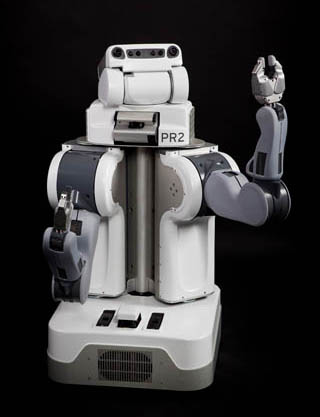
\includegraphics[height=8.0 cm]{PR2}
     \caption {PR2 service robot}
     \label {fig:PR2}
     \end {center}
     \end {figure}

 PR2 software is developed under ROS, an open source framework
for robot developers. ROS offers a collection of libraries ant tools, that helps creating
complex applications. The main ROS principle is collaboration, that improves
efficiency of the robotics software development. 

\section {Speech recognition software}
As speech recognition is a very popular field nowadays, there are numerous
software development projects, including open source, dealing with this area of
research. However, many of these projects are either in a test phase, or
intend for some special types of speech applications, support only particular
languages or not suitable for embedded systems, used for robot applications. 

 CMUSphinx, developed by Carnegie Mellon University, is
a leading speech recognition toolkit, that include a list of libraries and
toolkits, that allows solving various speech recognition tasks, including robot speech control.  The list of software tools includes:
\begin {itemize}
  \item 
Pocketsphinx — lightweight recognizer library written in C.
\item Sphinxbase — support library required by Pocketsphinx
\item Sphinx4 — adjustable, modifiable recognizer written in Java
\item CMUclmtk — language model tools
\item Sphinxtrain — acoustic model training tools
\item Sphinx3 — decoder for speech recognition research written in C
\citep{CMUSphinx}.
\end{itemize}
 \textit {Speech recognition} part of the project  uses Pocketsphinx and its depending library SphinxBase. The advantages
 of the choice are obvious:
 \begin {itemize}
   \item Pocketsphinx is resource-efficient, specially intended for embedded
   systems and thus perfectly suitable for robotics application
   \item Pocketsphinx is an open source
   \item Pocketsphinx is written in C, supports integration with Python 
   \item Pocketsphinx works with a number of ready-to-use high-quality
   language and acoustic models in a number of languages and allows models
   adaptation and training. 
 \end{itemize}
\section {Speech Recogniser Technical Requirements}
Speech recognition in robotics is characterised by a number of aspects in
comparison with a desktop speech recogniser. 

 First and one of the most serious problems is
background noise. Noise comes not only from the environment but also from the
motors of the robot.  To deal with the problem several strategies are used. 
These can be, for example, specific equipment for noise and echo reduction,
headsets for speakers, microphone arrays for robot, mounted ceiling microphones or a
combination of strategies. In our part of the project a headset is used to give
command to a PR2 robot.  The choice of the headset is also important. To improve
the quality of input signal a high-end noise canceling microphone is preferred. 

 Second, in robotics developers are often dealing with  a limited space and
computational efficiency. On the other hand, probabilistic search algorithms
require as a rule high computational efficiency. That is why realisation speech
recognition algorithms in a robotics environment demands  in some
cases adaptation of the algorithms to the robot environment.  In our
project Robot Operation System is used, including its libraries for speech
recognition, applicable for the purpose of efficiency optimisation.

Furthermore, sample rate is chosen as a rule as regulator of
input data amount and speech signal quality. For the project the sample rate is
equal 16 kHz or 16 bits/sample. The sound card should support 16-bit recording.
Which is a standard for the most sound cards. 

 Vocabulary
minimization and handling out of vocabulary word also improves performance of the application. 
The \textit{speech recognition} part of the project works with a limited number
of commands. The corpus consists of 12 sentences and 16 words. The number of 
sentences covers all executable commands of the application. It could have
been increased, when required, up to 50 words without any performance loss.
Bigger increase may require additional tuning of the application. 

All speech recognition systems are divided into speaker-independent and
speaker-dependent systems. 
Speaker-dependent systems are trained for a specific person and thus can achieve
better accuracy with a larger vocabulary. However, the systems have obvious
limitations in its usage.  In the \textit{speech recognition} part of the
project a speaker-independent approach is realised.  No training for a specific
person have been performed. 

Any speech recogniser implementation implies that it it technically possible for
a robot to follow speech commands. PR2 is equipped with all necessary
sensors that allow it to execute such instructions as
\textit {Pick up mug} or \textit{Go to table one}. Reactions to a stupid or
dangerous command should be reasonable. According to the application
scenario, PR2 ignore unknown commands, not coordinated with other project
groups. New command is not accepted till the previous command is not finished.
Manipulations with missing object are not allowed. This means, that the
execution of the commands like \textit {Pick up mug} or \textit {Bring mug to
counter} should be aborted, if the mug is not there. Proving of such conditions
should be done outside of the recogniser. When a command is recognised, PR2
asks for a confirmation. On the contrary, when a command is not recognised PR2
asks to repeat the command. 

\section {Design of  a statistical speech recogniser under ROS} 
\textit {Speech recognition} application starts  the following nodes: \textit
{recogniser}, \textit{talkback} and  \textit {soundplay}. The  nodes graph is shown in the figure ~\ref {fig:nodes}.  One more
node, shown here is  \textit {rosout}, that always runs and collects debugging
output from other nodes. 
\begin
 {figure}[h]
\begin {center}
     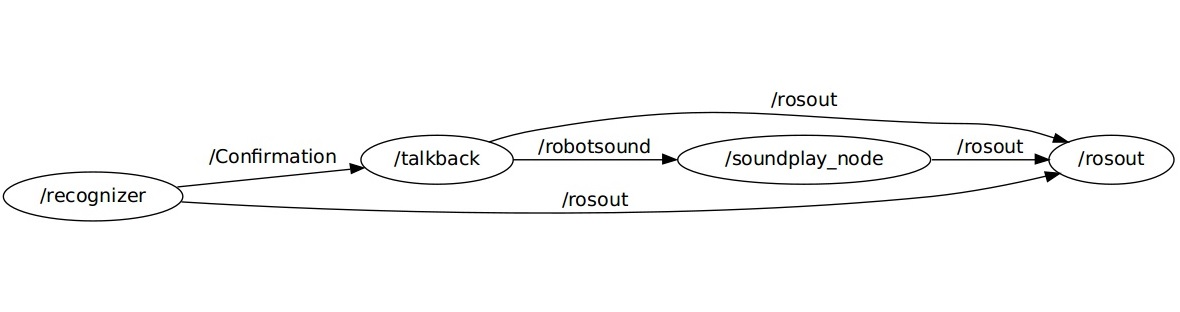
\includegraphics[height=4.0 cm]{nodes}
     \caption {Nodes graph of the recogniser application}
     \label {fig:nodes}
     \end {center}
     \end {figure}

 \textit {Recogniser} is a written in Python
ROS wrapper for Pocketsphinx library. \textit {Recogniser} becomes as input
parameters: language model, acoustic model and dictionary  with PR2
commands. Language model for the \textit {speech recognition} is built on
the basis on the Project corpus, containing PR2 control commands (see appendix ~\ref{app:commands}).
 As the number of commands is small, language model and dictionary are built
 automatically from the corpus, using online CMU Sphinx Knowledge Base
 tool. For larger models using of CMU language modelling toolkit is
 preferable.  Recogniser uses standard acoustic models. The most appropriate
 model for our application among available ones is general English acoustic
 model. 
 
\textit {Recogniser} is built on the basis of a \textit {Gstreamer}
media library. \textit {Gstreamer} is an open source streaming multimedia
framework, which enables playing and encoding of audio files. \textit
{Gstreamer} provides a pipeline for audio processing, where \textit {pocketsphinx}  plays a role of
a filter, that decode  a string message from an audio input. Encoded messages
are forwarded to the \textit {talkback} node for confirmation. Confirmed messages are sent via a message bus of the \textit {Gstreamer} to the
output rostopic \textit {Proj2013Command}. Encoded commands and search
information are printed in terminal (see figure \ref{fig:terminal}). 
\begin{figure}[h] 
\begin {center}
     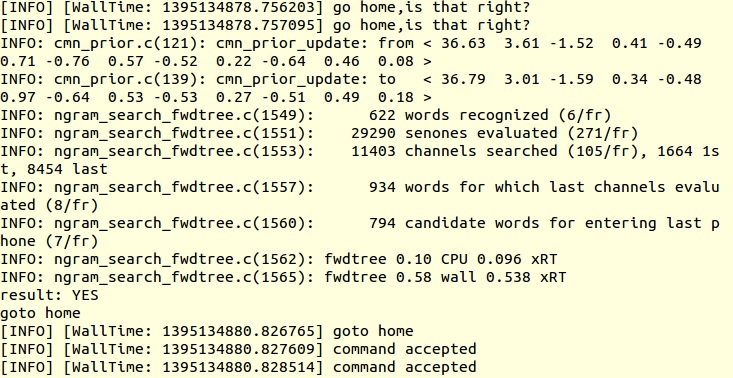
\includegraphics[height=8.0 cm]{terminal}
     \caption {Extract from the terminal output}
     \label {fig:terminal}
     \end {center}
     \end {figure}

 
\textit {Talkback} is a node, that initializes a feedback reaction
of the PR2 robot. It subscribes to the recogniser output and enables a play-back of the confirmation.
 Messages, meant for  a play-back, are forwarded to the
\textit {robotsound} topic for sound play.  Only confirmed messages are sent to
the \textit {Proj2013\_Command}. Interaction of \textit {talkback} and \textit
{recogniser} nodes are shown in the figure ~\ref {fig:mes}. 
\begin
{figure}[h] 
\begin {center}
     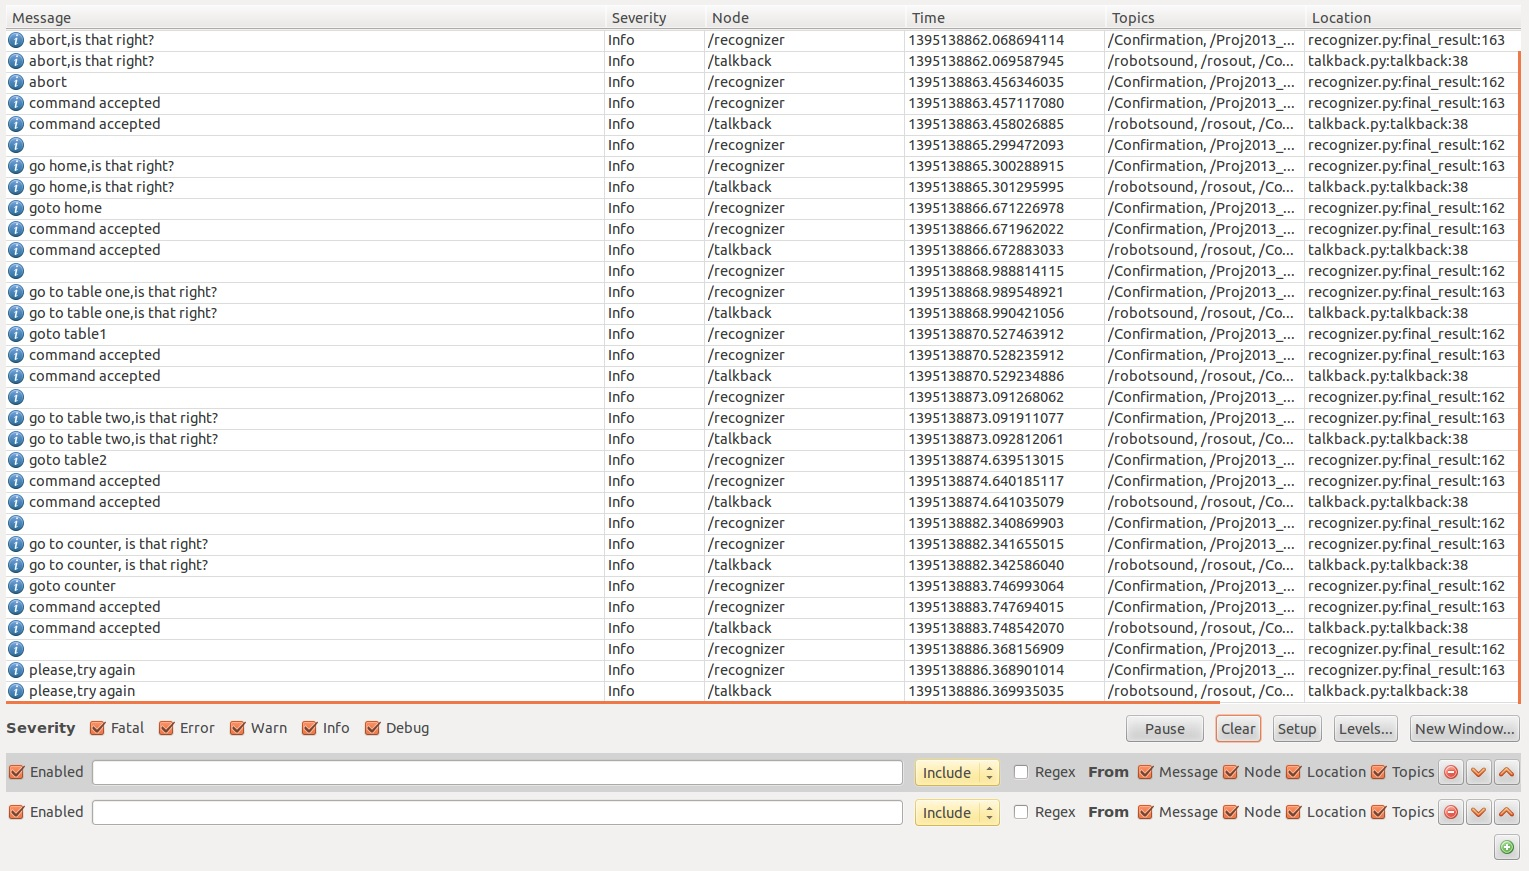
\includegraphics[height=8.0 cm]{commands}
     \caption {Messages, sent by Talkback and Recogniser }
     \label {fig:mes}
     \end {center}
     \end {figure}

 \textit {Soundplay} node subscribes to the \textit{robotsound
} topic and enables play-back of a message, using selected voice.
\textit{Soundplay} synthesizes speech from the messages received, using \textit
CMU \textit {Festival} Text-to-Speech library. Play-back is realised locally,
but for future there exist a possibility to realise a sound play-back via
a PR2 speaker.  

To sum it up,  \textit {speech recognotion} application is a simple speech
recogniser, that serves the purposes of the initial project specifications. It
is could be extended with other microphone configurations and used with
different language and acoustic models, including models, specially trained for
the situation. 

\chapter{Noise Reduction Techniques}
\label{sec:noise}

\section{Sound Source Separation}
\section{Spectral Substraction}

\chapter {Results}
\label {sec:results}
\section {Part 1}

\textit {Speech recognition} application was tested locally and after
integration as a part of the whole project application. Encoded commands have been published successfully in the
predefined format to the output and forwarded to PR2 for execution. 

 As a
recognition quality metric we have have used Word Error Rate (WER).  WER has the
following formula:
\begin {center}
$WER=\frac {S+D+I}N$, 
\end {center}
Where S is the number of substitutions, D is the number of
deletions, I is the number of Insertions and N is the total number of words.

 Accuracy calculation has been made on the basis of 20
repetitions of commands, stated in the corpus file (totally 37 words in 12 sentences). Computed figures 
serves only for approximate accuracy evaluation.  For detailed analysis more
sophisticated tests scenarios are necessary, involving greater number of
speakers and using test scripts and WER functions for support. 
\begin {table}[h]
\begin{center}
\begin{tabular}[h]{| c || c || c ||c || c|} \hline
Total words & S & D & I  & WER\\ \hline
740 & 18 & 3 & 12 & 0.45  \\
\hline
\end{tabular}
\caption {WER calculation of the Project speech recognition application}
\label {table:WER}
\end {center}  
\end {table} 

 
The results of the executed tests are presented in the table ~\ref{table:WER}.
As it can be seen from the above table most number of errors belong to the 
Substitutions. Instead of \textit {Go to counter} we get \textit {\textbf{No} to
Counter} or even \textit{\textbf {Mug} to counter}.  Resulted false utterances
are not fixed in the corpus file, but built by ASR as possible on the basis of
our corpus. \textit {Place mug to home},
shorted to \textit{Place mug home}, illustrates rarely occurred deletion.  One
more type of error is insertion. For example, a command
\textit {Go to table two} is changed to \textit {Go \textbf {up} to table two}. The most number of insertions happens at the end of the utterance (\textit {No}
vs. \textit {No \textbf {up}}, \textit {Abort} vs. \textit {Abort \textbf
{to}}). Such kinds of insertions are connected with mismatching of aspirations
at the end of an utterance with meaningful phonemes. The error of this type
are ignored by our application, if the whole preceding command is correctly
recognized. 

\begin {table}[h]
\begin{center}
\begin{tabular}[h]{| c || c || c|} \hline
Task & Vocabulary & Error rate \% \\ \hline
Digits & 11(zero-nine,oh)&0.5 \\
Wall Street Journal read speech & 5.000 &3 \\
Wall Street Journal read speech & 20.000 &3 \\
Broadcast news & 64.000+ &10 \\
Conversational telephone speech & 64.000+ &20 \\
Project ASR, using headset & 16 & up to 5\\
\hline
\end{tabular}
\caption {WER by speech recognition, based on particular scenarios}
\label {table:WERS}
\end {center}
\end {table}

Table \ref{table:WERS} shows different WERs of speech
recognition applications, depending on the environment and speech situation. As
it can be seen from the table the accuracy of the application is acceptable for
the application purposes, but it could be improved, taken into account, that we
are dealing with a limited vocabulary and using a headset.  

The nest step in accuracy improvement
would be tuning of the acoustic model by adapting it to the environment and training it,
using the  specified commands for audio records. Parallel other microphone
configurations (for example, built-in microphone) are preferably to be tested
for accuracy comparison.

\section {Part 2}

\chapter {Conclusion}
\label {sec:conclusion}

\section {Part 1}

In \textit {speech recognition} part of the Project we have
studied architecture of a modern speech recogniser and have presented detailed description of its
components and encoding technique.  Furthermore, we have analysed technical
requirements for a speech recogniser in robotics environment and  specifically
the possibilities of a speech recogniser realisation under ROS.
We have implemented a simple speaker-independent  speech recogniser under
ROS, based on specified for the Project 12 voice instructions, using default
acoustic model and command-based language model and dictionary. 

Our speech recognition application conforms with the projects
requirements and shows an acceptable WER of about 5 \%.  Moreover,
implemented speech recogniser is capable of being extended with other microphone
configurations, bigger vocabulary and adapted or trained acoustic
models according to the changed conditions. All the enumerated extension
possibilities create a serious basis for further project
research and implementation of sophisticated speech recognisers in PR2
environment.

\section {Part 2}

\begin{appendix}
\chapter {PR2 commands, used for speech control}
\label {app:commands}

\begin {itemize}
\item abort
\item go to counter
\item go to table one
\item go to table two 
\item go home
\item pick up mug 
\item place mug to counter
\item place mug to table one
\item place mug to table two
\item place mug to home
\end{itemize}

\end{appendix}

%\bibliographystyle{dinat}
\bibliographystyle{plain}
\bibliography{mybib,project}
 
\end{document}

